\section{Teoretický úvod}
  \indent
  \indent
  Dělič napětí nebo-li napěťoví dělič je elktrotechnické zapojení, které slouží k rozdělení napětí na $n$ částí, kde $n$ je počet impedancí v obvodu. Napěťové děliče můžeme rozdělit například na dvě skupiny:
  \begin{description}
    \item[Nezatížený napěťový dělič]
      \begin{figure}[htbp]
        \centering
        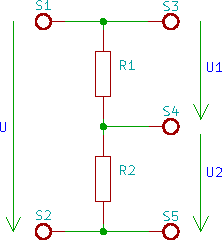
\includegraphics{../ne.pdf}
        \caption{Nezatížený napěťový dělič}
        \label{sch:ne}
      \end{figure}
      Jak je vidět ze schématu zapojení, tak nemá pžipojený zaťěžovací rezistor. Dá se popsat rovnicemi (1) a (2).

      \begin{equation}
        U_1 = U \cdot \dfrac{R_1}{R_1+R_2}
      \end{equation}


      \begin{equation}
        U_2 = U \cdot \dfrac{R_2}{R_1+R_2}
      \end{equation}
    
    \item[Zatížený napěťový dělič]
      \begin{figure}[htbp]
        \centering
        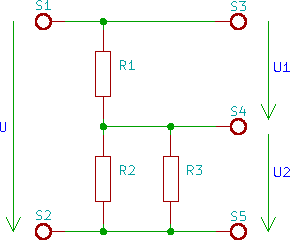
\includegraphics{../za.pdf}
        \caption{Zatížený napěťový dělič}
        \label{sch:ne}
      \end{figure}
      Jak již název napovídá má je tvořen nezatíženým napěťovím děličem a zatěžovacím rezistorem $R_3$. Dá se popsat rovnicemi (3) a (4).

      \begin{equation}
        U_1 = U \cdot \dfrac{R_1}{R_1+ \dfrac{R_2 R_3}{R_2+R_3}}
      \end{equation}


      \begin{equation}
        U_2 = U \cdot \dfrac{\dfrac{R_2 R_3}{R_2+R_3}}{R_1 + \dfrac{R_2 R_3}{R_2+R_3}}
      \end{equation}
  \end{description}
